\section{Validation du design}
Lors de cette section, sera décrite la procédure de vérification des caractéristiques du projet ainsi la validation de celui-ci.
\subsection{Liste de matériel} \label{ssec:ListeMateriel}
{
	\begin{enumerate}
		\item Oscilloscope Tektronix RTB2004 ES.SLO2.05.01.16 \label{enum:oscillo}
		\item USB Logic Analyzer, 8-Canaux, 24MHz \label{enum:logicAnalyzer}
		\item USB TO TLL HW-597 \label{enum:USB-TTL}
		\item Carte Localisation-Sous-Marine V0.0 \label{enum:PCBL}
	\end{enumerate}
}

\subsection{Contrôle des alimentations}
{
	En premier lieu, une vérification des tensions d'alimentation permet de valider un aspect critique et fondamentale de la carte.
	\subsubsection{Méthodologie}
	\paragraph{Mesure du 3.3V :} Alimentation de la carte par une connections brève entre les pins du connecteur du bouton \textbf{P15}. Mesure sur le testpoint \textit{V\_regOUT5} voir figure \ref{fig:sch3}.
	\begin{figure}[h]
		\centering
		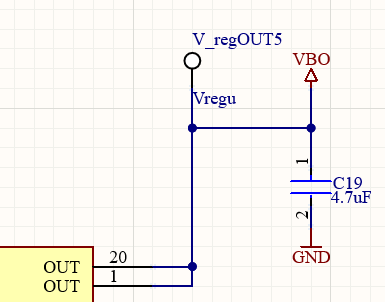
\includegraphics[width=0.3\linewidth]{Figures/DEV_MEAS/Sch3.3V}
		\caption{Testpoint mesure 3.3V}
		\label{fig:sch3}
	\end{figure}
	
	\paragraph{Mesure du 5V :} Pour mesurer le 5V, il faut ponter par une résistance $0\Omega$ la résistance R50, ainsi que activer la Pin RC5 / EN\_5V. Ensuite la mesure a été prise sur le connecteur P16, pin-3 :
	\begin{figure}[h]
		\centering
		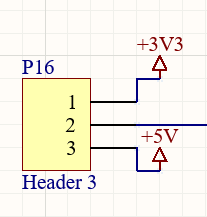
\includegraphics[width=0.2\linewidth]{Figures/DEV_MEAS/Sch5V}
		\caption{Schéma de mesure 5V}
		\label{fig:sch5v}
	\end{figure}

	\clearpage
	
	\subsubsection{Mesures}
	
	\begin{figure}
	\begin{subfigure}{.5\textwidth}
		\centering
		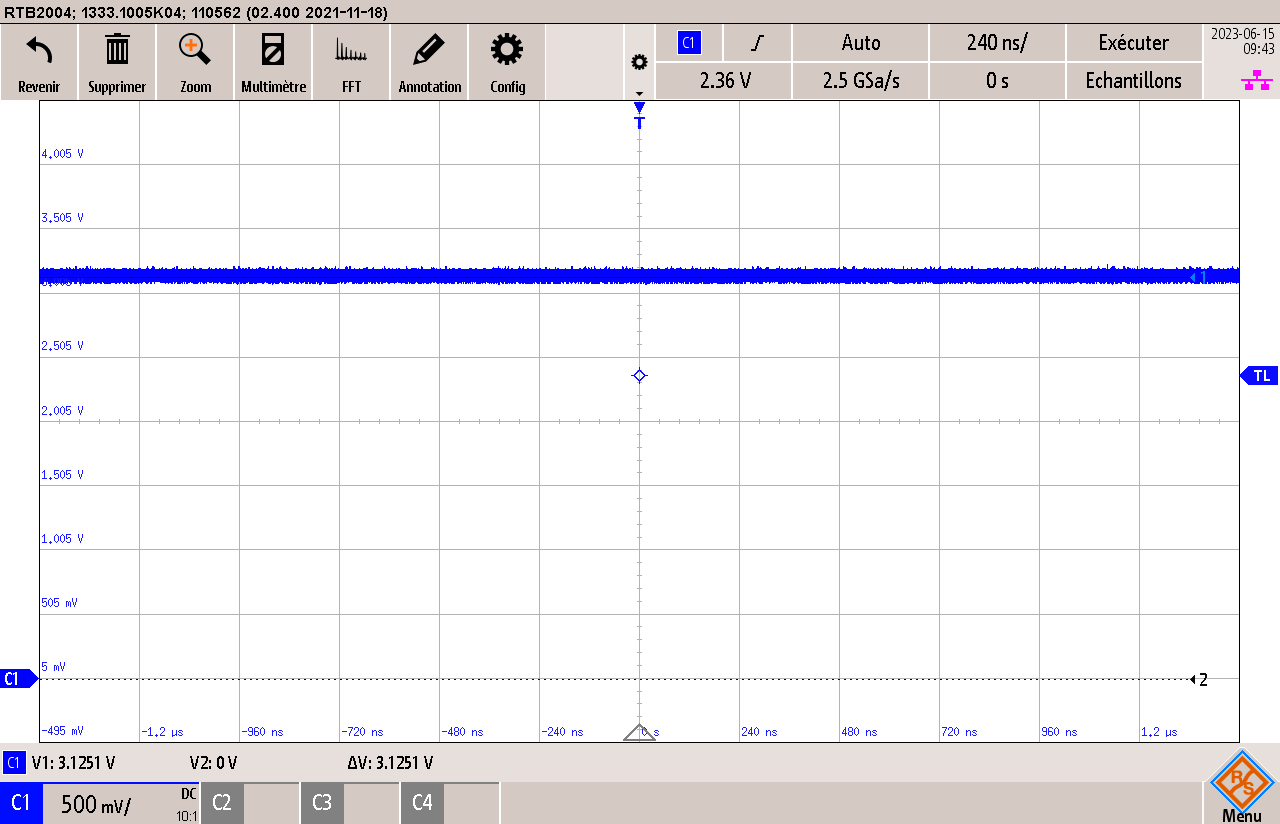
\includegraphics[width=\textwidth]{Mesures/Tension3.3V}
		\caption{Mesure 3.3V}
		\label{fig:Mes3.3V}
	\end{subfigure}
	\begin{subfigure}{.5\textwidth}
		\centering
		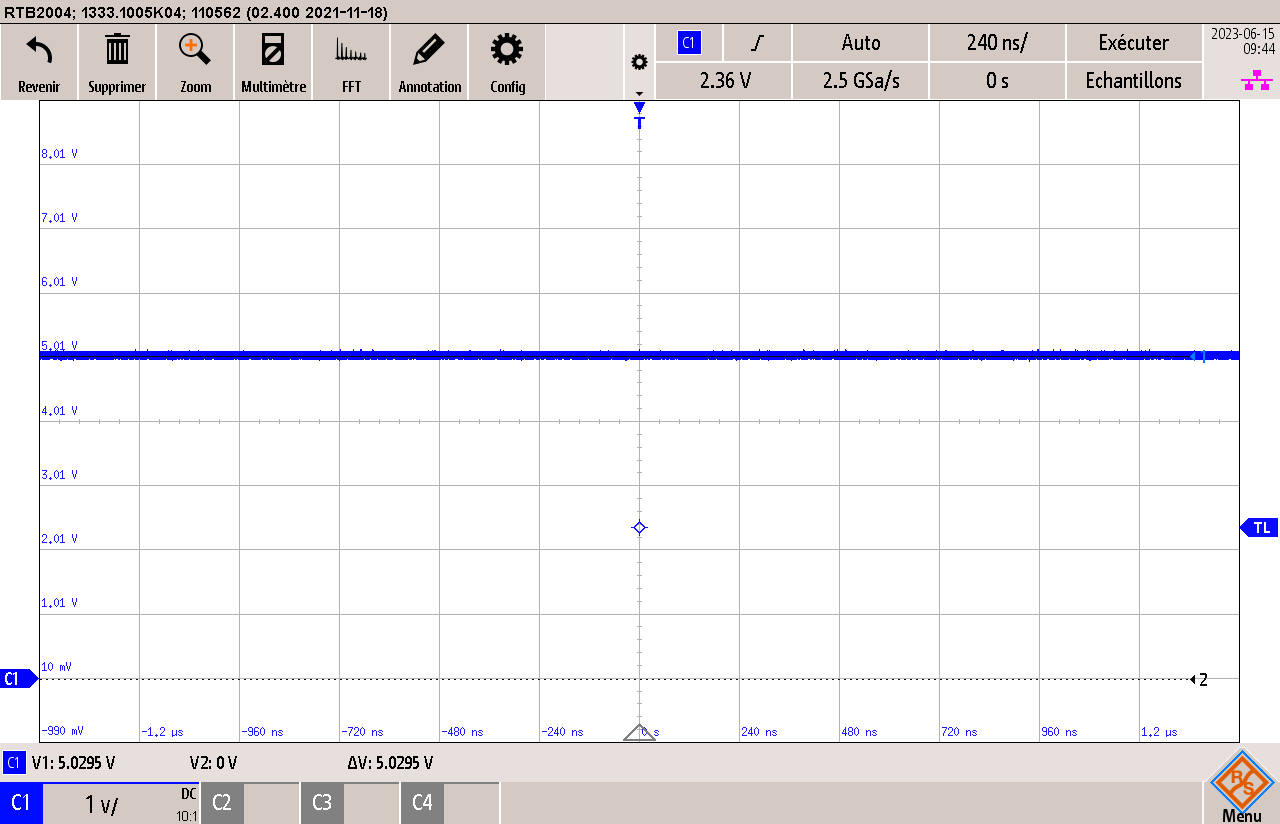
\includegraphics[width=\textwidth]{Mesures/Tension5V}
		\caption{Mesure 5V}
		\label{fig:Mes5V}
	\end{subfigure}
	\caption{Mesures des tensions d'alimentations}
	\label{fig:Mesure3.3et5V}
	\end{figure}
	
	\paragraph{Analyse :} Nous pouvons observer les valeurs respective des tensions sur les figures \ref{fig:Mes3.3V} et \ref{fig:Mes5V}. La tension d'alimentation du microcontrôleur est mesurée à \textit{3.125V} ce qui peut être expliqué par une chute de tension aux bornes de la batterie LI-ION qui par conséquent à besoin d'être chargée. La tension 3.3V oscille légèrement, ceci peut s'expliquer par le fait qu'il s'agit de l'alimentation principale de la carte avec le plus de consommateurs. Mais également par le fait que des signaux rapides sont générés par le microcontrôleur et ses différents périphériques.
	
	La tension d'alimentation du capteur de pression dont la tension dimensionnée est de 5V est quant-à-elle mesurée à \textit{5.0295V} ce qui signifie une bonne précision de la part du circuit de boost. On peut également voir que la tension n'oscille pas et ne vas donc pas perturber le capteur de pression.
	
	Nous pouvons donc confirmer le fonctionnement des blocs d'alimentation du projet.
	
}

\subsection{Communication UART}
{
	Comme décrit lors de la sous-section \ref{ssec:Usart} une communication série est implémenté dans projet. Cette communication n'est pas critique pour le projet mais il est important de vérifier son fonctionnement pour d'éventuelles versions ultérieures.
	\subsubsection{Méthodologie}
	Pour la mesure, l'analyseur logique (Numéro \ref{enum:logicAnalyzer} de la liste de matériel \ref{ssec:ListeMateriel}) a été utilisé. Les trames U1TX et U1RX ont été mesurée sur le connecteur P4 :
	
	\begin{figure}[h]
		\centering
		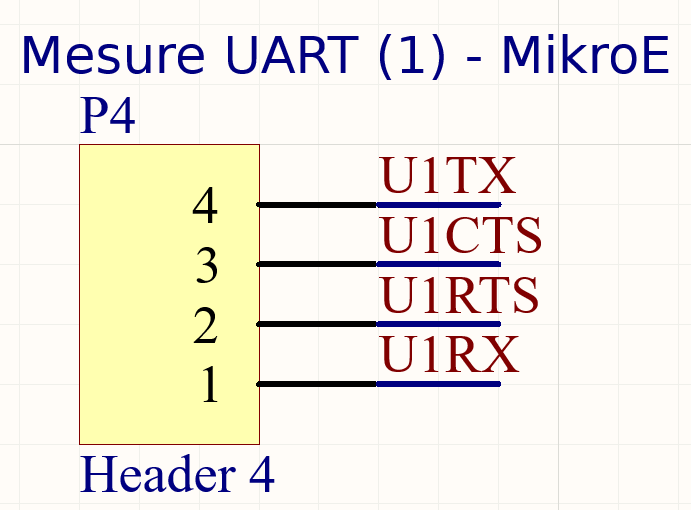
\includegraphics[width=0.2\linewidth]{Figures/DEV_MEAS/SchUart1}
		\caption{Schéma de mesure UART1}
		\label{fig:schuart1}
	\end{figure}
	\clearpage	
	\subsubsection{Mesures}
	
	\begin{figure}[h]
		\centering
		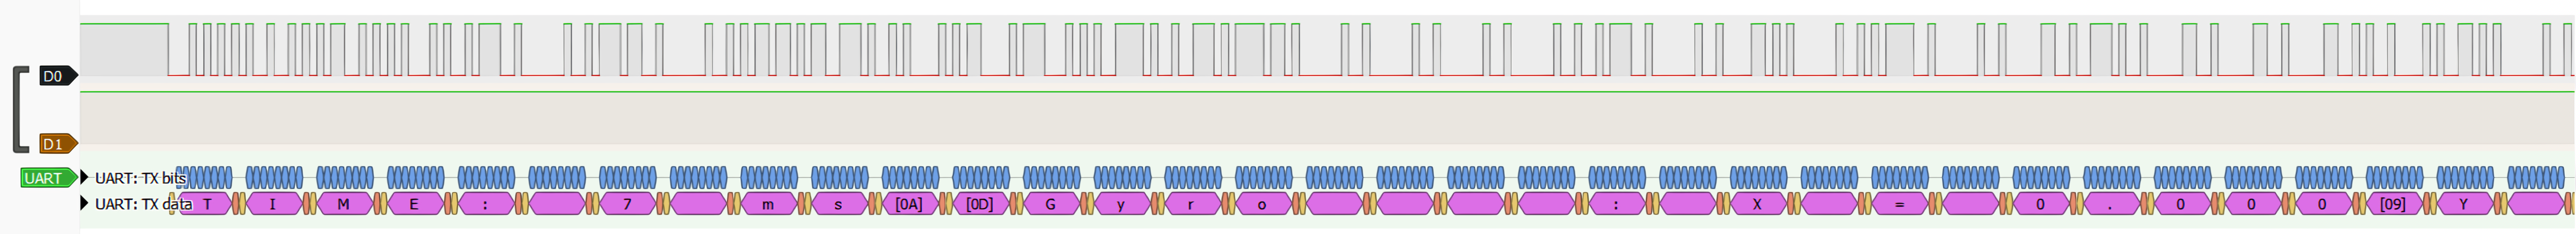
\includegraphics[width=1.1\linewidth]{Mesures/MesureTrameUart_Upscaled}
		\caption{Mesures trames UART}
		\label{fig:mesuretrameuart}
	\end{figure}

	\paragraph{Analyse :} On peut lire en caractères ascii sur la trame de la figure \ref{fig:mesuretrameuart} : 
	\begin{lstlisting}[frame=single, caption={Trame UART en ASCII}, captionpos=b, breaklines=true]
TIME: 7 ms 
Gyro    : X = 0.000	Y 
	\end{lstlisting} 

	En connectant le module USB-TO-TTL (Numéro \ref{enum:USB-TTL} de la liste de matériel \ref{ssec:ListeMateriel}) au broches Tx et Rx de la figure \ref{fig:mesuretrameuart}. Puis en ouvrant une communication série via PuTTY à un bauderate 115200. On obtient la communication de la figure \ref{} dans la console :
	
	\begin{figure}[h]
		\centering
		\fbox{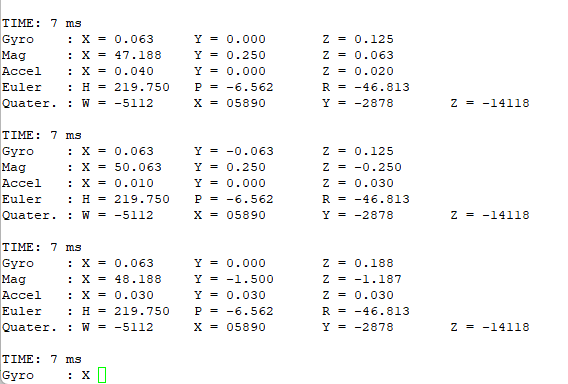
\includegraphics[width=0.7\linewidth]{Mesures/PuttYSerComm}}
		\caption{Récéption UART PuTTY}
		\label{fig:puttysercomm}
	\end{figure}
	
	

}

\subsection{Communication SPI, carte SD}
{
	\subsubsection{Méthodologie}
	
	\subsubsection{Mesures}

}

\section{Caractéristiques du produit finis}

% J'ai pus sans difficulté faire un logging sur 5h et ai récolté 30MB de données dans le fichier CSV, ce qui correspond aux $\sim5$ heures de logging
